\documentclass{article}
\usepackage{amsmath}
\usepackage{tikz}
\usetikzlibrary{matrix}

\begin{document}

\begin{figure}[h]
    \centering
    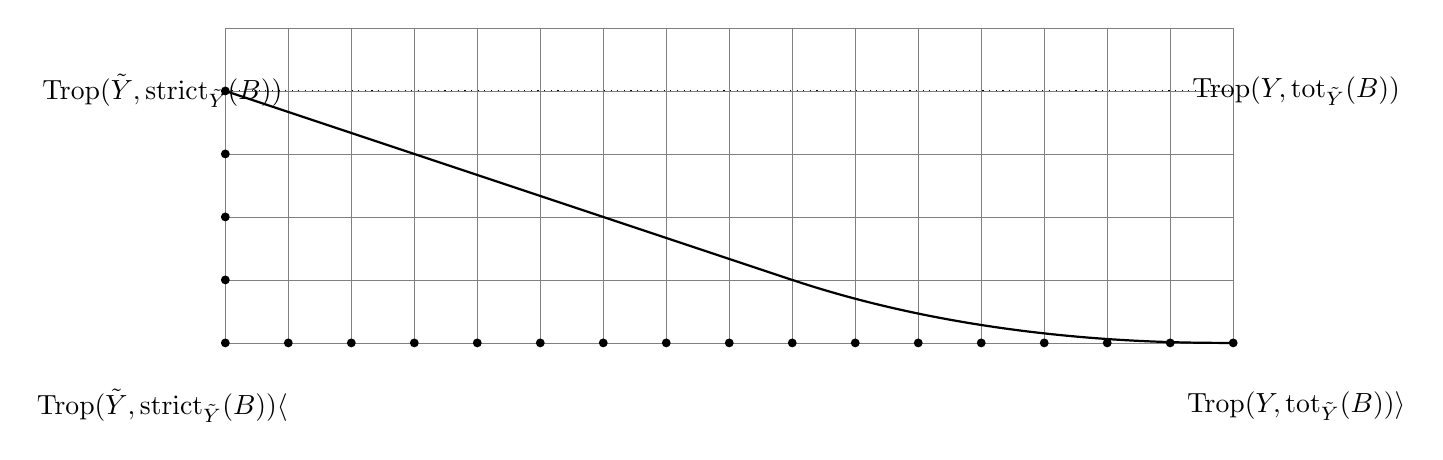
\begin{tikzpicture}[scale=0.8]
        % Draw the grid
        \draw[help lines] (0,0) grid (16,5);
        
        % Draw the dotted line
        \draw[dotted] (0,4) -- (16,4);
        
        % Draw the points
        \foreach \x in {0,...,16} {
            \fill (\x,0) circle (2pt);
        }
        \foreach \y in {1,...,4} {
            \fill (0,\y) circle (2pt);
        }
        
        % Draw the curve
        \draw[thick] (0,4) .. controls (3,3) and (6,2) .. (9,1) .. controls (12,0) and (15,0) .. (16,0);
        
        % Labels
        \node at (-1,4) {$\mathrm{Trop}(\tilde{Y},\mathrm{strict}_{\tilde{Y}}(B))$};
        \node at (17,4) {$\mathrm{Trop}(Y,\mathrm{tot}_{\tilde{Y}}(B))$};
        \node at (-1,-1) {$\mathrm{Trop}(\tilde{Y},\mathrm{strict}_{\tilde{Y}}(B))\langle$};
        \node at (17,-1) {$\mathrm{Trop}(Y,\mathrm{tot}_{\tilde{Y}}(B))\rangle$};
    \end{tikzpicture}
    \caption{Graphical summary of $\mathbb{P}(1,1,4)$, Case II. When the integer point $(0,4)$ is missing from $\mathrm{Newt}(\Omega)$, we move the edge corresponding to the exceptional divisor of the minimal resolution $\mathbb{F}_4\to\mathbb{P}(1,1,4)$ normally inwards until it reaches an integer point. The new edge has affine length $4$, which implies that the strict transform of the branch curve intersects the contracted $-4$-curve $C_1$ with total multiplicity $4$. The affine distance from the missing point to the new edge is $1$, so the curve $C_1$ appears in $\mathrm{tot}_{\tilde{Y}}(B)$ with multiplicity $1$.}
    \label{fig:summary}
\end{figure}

\end{document}